\documentclass{ujarticle}
\usepackage{ketpic,ketlayer}
\usepackage{amsmath,amssymb}
\usepackage{graphicx}
\usepackage{xcolor}
\usepackage{bm,enumerate}
\usepackage[dvipdfmx,colorlinks=true,urlcolor=blue]{hyperref}

\setmargin{20}{15}{15}{15}

\西暦

\renewcommand{\labelitemi}{・}
\pagestyle{empty}

\begin{document}

\begin{center}
KeTCindyのインストール
\end{center}

\vspace{-5mm}

\hfill 修正日:\today

\begin{enumerate}[\bf\large 1.]
\item Cinderella, R, Maxima とSumatra(Windowsのみ)をインストールする.\vspace{-2mm}

 \begin{itemize}
 \item \url{https://beta.cinderella.de}  (Cinderella)\\
\hspace*{6mm}注)Windowsの場合,右クリックして「管理者として実行」を選ぶ.
 \item \url{https://cran.r-project.org}   (R)
 \item \url{https://sourceforge.net/projects/maxima/files}  (Maxima)
 \item \url{https://www.sumatrapdfreader.org/download-free-pdf-viewer.html} (Sumatra)\\
\hspace*{6mm}注)Sumatraのインストール先は,オプションでProgram Files(またはx86)を指定する.

 \end{itemize}
\item TeXをインストールしていない場合はインストールする.\vspace{-2mm}
 \begin{enumerate}[(1)]
 \item TeXLiveを推奨 (2018以降ではketcindyが組み込まれている)
 \item KeTTeXはTeXLiveの軽量版で以下からダウンロードできる.\\
    \hspace*{5mm}Mac (kettex.dmg)\\
    \hspace*{10mm}\url{https://www.dropbox.com/s/dc4inuk06t07g26/kettex.dmg?dl=0}\\
    \hspace*{5mm}Windows (kettex.exe)\\
    \hspace*{10mm}\url{https://www.dropbox.com/s/fthw4btjqqs33tc/kettex.exe?dl=0}\\
    \hspace*{5mm}Linux (kettex.tar.xz)\\
    \hspace*{10mm}\url{https://www.dropbox.com/s/vg8p07832e9hzlk/KeTTeX-linux-20171022.tar.xz?dl=0}\\
    \hspace*{5mm}注)解凍したkettexの保存先 /Application\ (Mac), C:\textbackslash\ (Windows)\\
    \hspace*{5mm}注)Mac(Catalina)の場合,ターミナルで \verb|spctl --master-enable| を実行

\end{enumerate}
 
\item KeTCindyのインストール\vspace{-2mm}
  \begin{enumerate}[(1)]
  \item ketcindyをCTAN(\url{https://ctan.org})からダウンロードする.\\
  \hspace*{10mm}ketcindyで検索 $>$ Package ketcindy $>$ Download(フォルダ名はketcindy)
    \begin{itemize}
    \item Repositoryはgithubサイトにある最新版へのリンク\\
        \hspace*{10mm}Clone or download $>$ Download ZIP(フォルダ名はketcindy-master)          
     \end{itemize}
  \item Mac,Linuxの場合は,最初にフォルダ内の\verb|ketcindykc|をCtrL+クリックで実行する.
  \item \verb|ketcindysettings.cdy|をダブルクリック,以下の(1)(2)を選択して,(3)を順に実行する.
    \begin{itemize}
    \item 必要なら,実行プログラムをCinderellaに設定する.
    \item 他のcdyファイルを開いているときは,Cinderellaを一旦終了してからにする.
   \item 画面が狭ければ,右方向に広げる.
   \end{itemize}

\vspace{3mm}

\begin{layer}{140}{0}
\putnotese{7}{20}{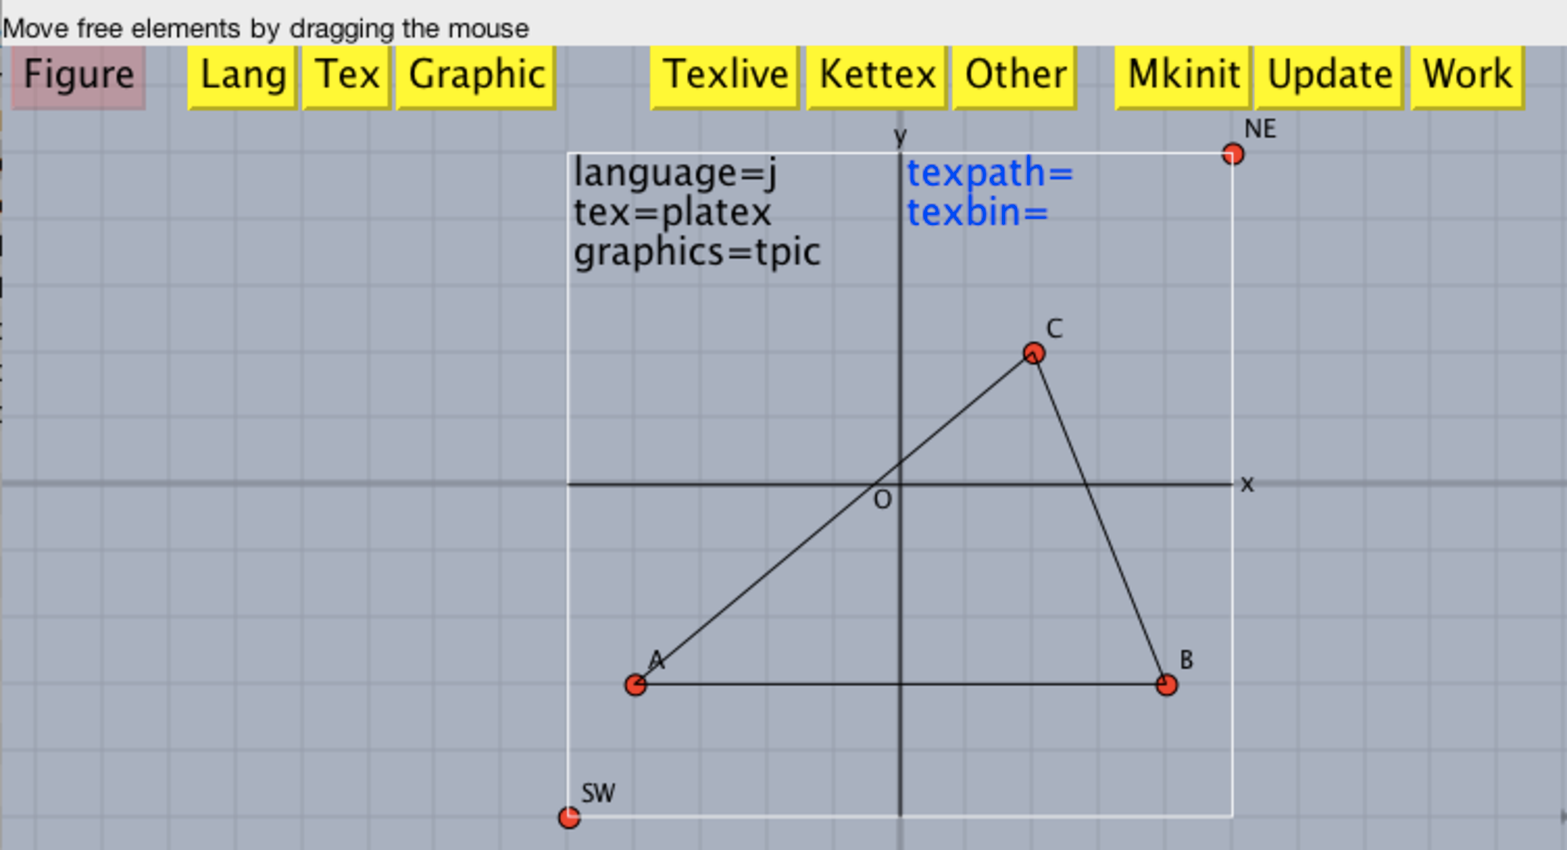
\includegraphics[bb=0.00 0.00 752.00 408.00,width=100mm]{Fig/setting.pdf}}
\putnotee{-20}{5}{\bf [1]\ 言語などの選択}
\putnotese{-17}{10}{\underline{Language}}
\putnotese{-13}{15}{Japanese, English}
\putnotese{-17}{20}{\underline{\TeX}}
\putnotese{-15}{24}{\begin{tabular}{l}
platex\\uplatex\\latex\\xelatex\\pdflatex\\lualatex\end{tabular}}
\putnotese{-17}{58}{\underline{Graphic Code}}
\putnotese{-15}{62}{\begin{tabular}{l}tpic\\pict2e\\tikz\end{tabular}}
\arrowline{27}{20}{20}{135}
\putnoten{63}{7}{\bf [2]\ \TeX システムの選択}
\arrowline{63}{20}{13}{90}
\putnotee{105}{5}{\bf [3]\ 作成と更新}
\arrowline{90}{20}{20}{45}
\putnotese{111}{9}{\fbox{Mkinit}}
\putnotese{113}{15}{\begin{minipage}[t]{52mm}%
初期設定ファイルketcindy.iniをユーザホーム(ホーム)に作成
\end{minipage}}
\putnotese{111}{26}{\fbox{Update}}
\putnotese{113}{32}{ketcindyを更新}
\putnotese{110}{37}{\begin{minipage}[t]{52mm}%
{\color{red}「実行不可」が出た場合}\\
\hfill(Mac,Linuxで初回のみ)\\
\hspace*{3mm}ターミナルを立ち上げて\\
\hspace*{5mm}cd (figフォルダをDrag\&Drop)\\
\hspace*{5mm}chmod 777 kc.command(sh)
\end{minipage}}
\putnotese{111}{64}{\fbox{Work}}
\putnotese{113}{70}{\begin{minipage}[t]{52mm}%
作業フォルダketcindyをホームに作成\\
\hspace*{3mm}マニュアルやサンプルなど
\end{minipage}}
\end{layer}

\vspace{77mm}

{\bf [4]\ テストラン}

\begin{itemize}
 \item 最初は図が出ないが,設定が完了すると図が表示される.
\item\verb|Figure|を押して,pdfが表示されれば成功
\end{itemize}

  \end{enumerate}

\end{enumerate}

\end{document}